\section{Network Choice}
\label{sec:network_choice}

The network choice is a very important aspect of the project, because it
defines the limitations and the costs of the system. We want to aim for a
blockchain that has low fees, is fast, secure and scalable, and since this is
done using solidity, we have to aim for an EVM compatible network. To see which
network matches our requirements, we need to analyze the statistics of the most
popular EVM compatible networks, because these are the more secure ones.

Following Figure~\ref{fig:network_comparison}, we can see the main differences
between the networks with the highest transactions per second (TPS). The main
aspects to take into account from this Figure are the TPS and the finality.

\begin{figure}[H]
    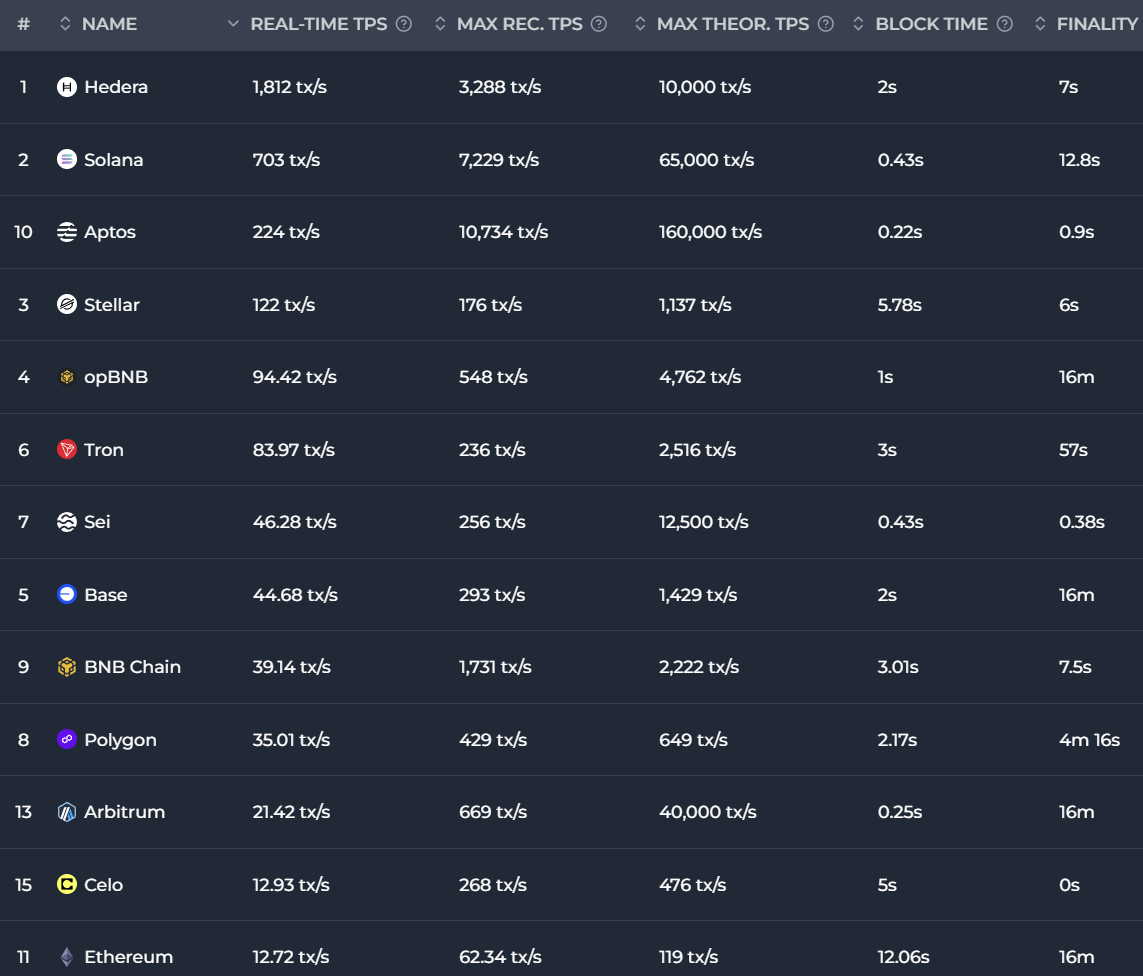
\includegraphics[width=\textwidth*2/3]{Network comparison 1.png}
    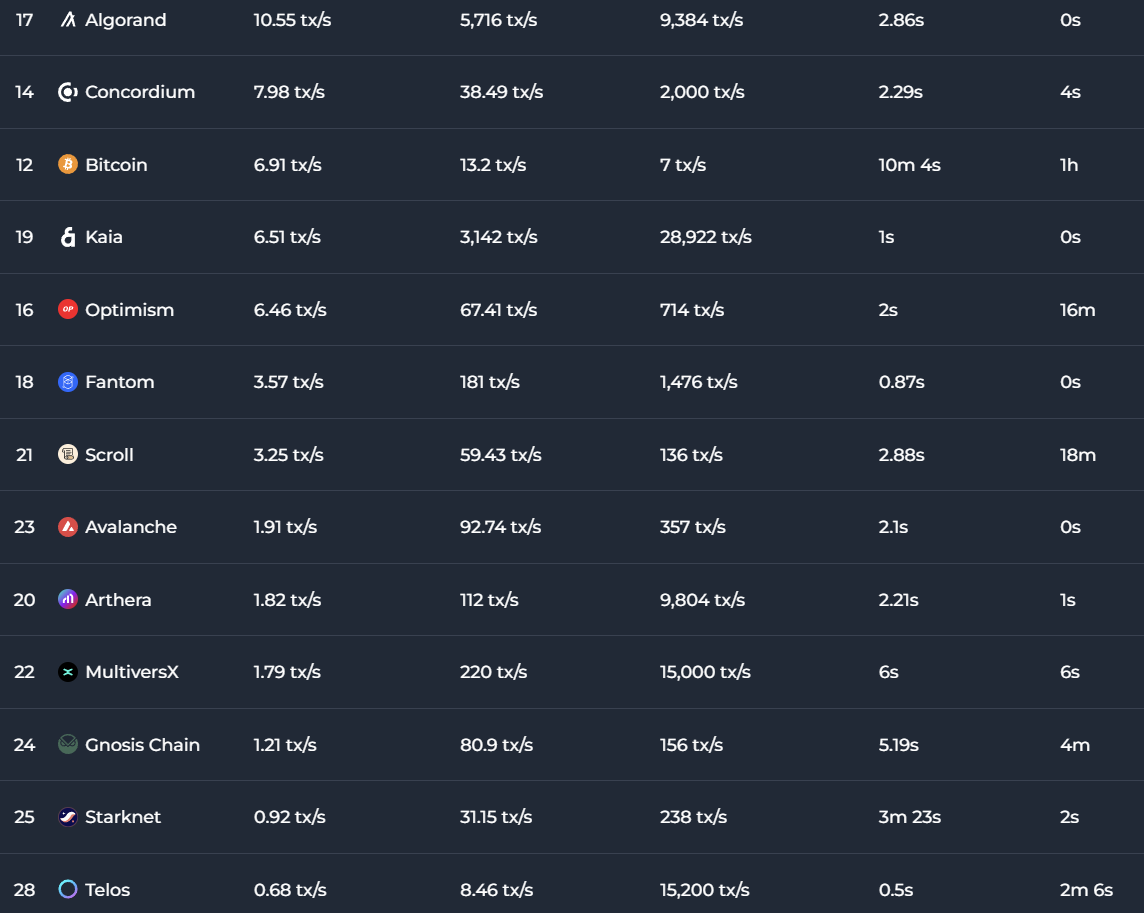
\includegraphics[width=\textwidth*2/3]{Network comparison 2.png}
    \centering
    \caption{Network comparison. Extracted from ...}
    \label{fig:network_comparison}
\end{figure}

Blockchains with higher TPS means they are more scalable, meaning they can
process that amount of transactions in one second. Similar to how Visa and
Mastercard work, they can process thousands of transactions per second, so the
users don't have to wait for a long time for the transaction to be processed.
In our case, a high TPS is important, but even more is the finality.

The finality is the time it takes for a transaction to be fully registered on
the blockchain, meaning the time it takes for the transaction to be
irreversible. This is important because we want the users to be able to enter
the event as soon as possible, so the transaction to validate the tickets must
be as fast as possible. This is the value that, if it takes too long, we will
be waiting for each user individually to enter the event, which would be a
problem. It's possible to see Ethereum down there, which has an average of 16
minutes for the finality, which is way too much for what we need.

Unfortunately a lot of networks there are not EVM compatible, so we have to
choose between the ones that are. The two options that we could consider are
the BNB Chain (also known as Binance Smart Chain (BSC)) and the Avalanche,
being the first one the most popular and with higher scalability, but the
second one has a way better finality.

The Avalanche chain would be the best bet, but having close to 2 tx/s
(transactions per second), maybe its not scalable enough. For the BSC, it has a
good enough finality and a good TPS so it would be a good choice for the
project. This chain is also very popular and was created by Binance, one of the
biggest companies in the blockchain ecosystem, so it's very secure and
reliable.

\subsection{Fees}
\label{subsec:fees}

With this in mind, we still need to take into account the network fees. If this
chain had high fees, then we would be forced to switch to another. Luckily, the
BSC has very low fees, as Figure~\ref{fig:network_fees} shows, being the peak
at 0.50 USD. Note that these are the fees to pay for a transaction, so if a
user wants to buy multiple tickets, he can make it all at once instead of
several individual purchases.

\begin{figure}[H]
    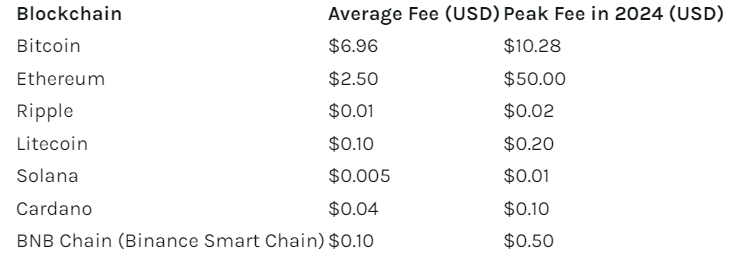
\includegraphics[width=\textwidth*2/3]{Network fees.png}
    \centering
    \caption{Network fees. Extracted from ...}
    \label{fig:network_fees}
\end{figure}

These fees are necessary as they are the cost for making the network run. This
is common in the blockchain ecosystem, and it's a way to maintain the network
secure and reliable, because the people processing the transactions are
rewarded for their work, so they have an incentive to keep the network running.
So we can never run away from this kinds of fees, but we can choose networks
that have lower fees, so the users pay the least amount possible.
